\documentclass{article}

\usepackage{arxiv}

\usepackage[utf8]{inputenc}
\usepackage[T1]{fontenc}
\usepackage{hyperref}
\usepackage{url}
\usepackage{booktabs}
\usepackage{amsfonts}
\usepackage{nicefrac}
\usepackage{microtype}
\usepackage{graphicx}
\usepackage{amsmath,amssymb,mathtools}
\usepackage{multirow}
\usepackage{subcaption}
\usepackage{algorithm}
\usepackage{algorithmic}

\title{HDML: Hierarchical Decision Mamba-Liquid Architecture for Multi-Embodiment Continuous Robotic Control}

\author{
  HDML Research Initiative \\
  Autonomous Control \& Foundation Models Team \\
}

\date{\today}

\begin{document}
\maketitle

\begin{abstract}
High-dimensional continuous control in multi-articulated robotic systems---ranging from quadrupeds and 3D humanoids to serpentine and bipedal mechanisms---faces a fundamental multi-scale challenge: reconciling long-horizon macro-cognitive reasoning over temporal state-action trajectories with high-frequency, continuous-time motor execution on physical actuators. While discrete Transformer-based sequence models capture long-term behavioral dependencies, they incur quadratic computational complexity $\mathcal{O}(T^2)$, exhibit severe vulnerability to distribution shifts under physical perturbations, and induce high-frequency torque chatter. To overcome these limitations, we propose \textbf{HDML} (\textbf{H}ierarchical \textbf{D}ecision \textbf{M}amba-\textbf{L}iquid), a generalist multi-embodiment foundation architecture. HDML couples a native Selective State Space Model (\textbf{Mamba-3}) backbone with built-in rotary state embeddings (RoPE) and trapezoidal discretization for $\mathcal{O}(1)$ streaming inference with an Optimal Transport Flow Matching action-chunk policy and a continuous-time Closed-Form Continuous-Time (\textbf{CfC}) Neural ODE motor filter for chatter-free actuator control. Pre-trained across 11 diverse robotic morphologies comprising exactly 1,735,673 physical transitions in MuJoCo, HDML demonstrates rapid few-shot transfer: freezing 11.61M backbone parameters (92.8\%--93.9\%) while adapting lightweight Universal Embodiment Adapters in under 30 seconds yields an action prediction loss of $0.00602$ on a 12-DoF Unitree A1 quadruped and $0.02579$ on a 17-DoF 3D Humanoid. Under continuous sensor noise and random external force impulses, HDML maintains a robust Interquartile Mean (IQM) score of \textbf{10.24} [8.44, 13.72] with 100\% episode survival, achieving an \textbf{8.7$\times$} performance retention over Decision Transformer ($1.17$) and outperforming Decision RNN ($7.91$). Furthermore, HDML achieves the lowest mechanical jerk among sequence models ($0.5724$ vs. $0.8109$ for DT, a 29.4\% reduction) while sustaining a pure inference latency of \textbf{8.14 ms} (\textbf{122.9 Hz}) and an end-to-end closed-loop control frequency of \textbf{110.8 Hz} (\textbf{9.02 ms} total cycle including physics simulation and PACE safety monitoring) on an NVIDIA RTX 4070 SUPER GPU.
\end{abstract}

\keywords{Continuous Robot Control \and Multi-Embodiment Foundation Model \and Selective State Space Models \and Liquid Neural Networks \and Flow Matching \and Offline Reinforcement Learning}

\section{Introduction}
\label{sec:intro}

The emergence of sequence modeling paradigms in offline reinforcement learning, epitomized by Decision Transformers (DT) \cite{chen2021decision} and trajectory diffusion policies \cite{chi2023diffusion}, has reframed continuous robotic control as conditional autoregression over sensory-action tokens. However, when deployed onto multi-articulated physical embodiments---such as quadrupedal robots (e.g., Unitree A1), 3D bipedal humanoids, and agile manipulators \cite{zhao2023learning, brohan2023rt2}---standard discrete autoregressive architectures encounter three critical theoretical and computational barriers:

\begin{enumerate}
    \item \textbf{The Temporal Scale Dichotomy:} High-level behavioral planning operates over macroscopic horizons (e.g., $1$--$5\text{ Hz}$ cognitive intent), whereas joint torque actuation requires high-frequency closed-loop execution ($50$--$500\text{ Hz}$) to reject physical disturbances and maintain dynamic balance.
    \item \textbf{Actuator Smoothness and Mechanical Jerk:} Standard feedforward and attention-based policies output discrete step-to-step action jumps, inducing high mechanical jerk $\mathcal{J} = \frac{1}{T}\sum_t \|\Delta^2 a_t\|_2$. External low-pass filtering introduces phase lag and non-Markovian dynamics, degrading closed-loop stability and causing premature motor fatigue.
    \item \textbf{Covariate Shift under Perturbations:} Self-attention over past context histories exhibits high sensitivity when unexpected external force impulses or sensor noise induce distribution shifts, leading to compounding autoregressive errors and catastrophic policy failure.
\end{enumerate}

To resolve this multi-scale dichotomy, we introduce \textbf{HDML} (\textbf{H}ierarchical \textbf{D}ecision \textbf{M}amba-\textbf{L}iquid), a unified architecture bridging macroscopic sequence reasoning and microscopic continuous-time dynamics. HDML establishes a dual-rate hierarchy: a native Selective State Space Model (\textbf{Mamba-3}) backbone \cite{gu2023mamba} with built-in rotary state-space embeddings and trapezoidal integration processes multi-modal state-return tokens with linear $\mathcal{O}(T)$ training and $\mathcal{O}(1)$ streaming complexity. Action chunks are generated via Optimal Transport Flow Matching \cite{lipman2023flow}, while an analytical Closed-Form Continuous-Time (\textbf{CfC}) Neural ODE head \cite{hasani2022closed, lechner2020neural} smooths high-frequency motor actuation and dampens physical disturbances directly in the continuous-time domain.

\paragraph{Summary of Contributions:}
\begin{itemize}
    \item \textbf{Hierarchical Mamba-Liquid Architecture:} We formulate a dual-timescale foundation model coupling native Mamba-3 Selective State Space Models with Optimal Transport Flow Matching and continuous-time Liquid ODE filters.
    \item \textbf{Universal Multi-Embodiment Pre-training:} We pre-train HDML across 11 distinct physics morphologies (exactly 1,735,673 transitions) using zero-copy pinned GPU memory buffers, achieving a $13.85\times$ data throughput speedup (reducing epoch duration from 18 minutes to 78 seconds).
    \item \textbf{Parameter-Efficient Few-Shot Transfer:} By freezing 92.8\%--93.9\% (11.61M) of core backbone parameters, HDML adapts to novel embodiments (Unitree A1, Humanoid 3D, Swimmer, Ant, Hopper, Walker2d) via lightweight Universal Embodiment Adapters in under 30 seconds.
    \item \textbf{Rigorous Perturbation Robustness \& Smooth Actuation:} Under random force impulses ($F=50\text{ N}$) and sensor noise, HDML maintains an IQM score of \textbf{10.24} (100\% survival rate), outperforming Decision Transformer ($1.17$, an 8.7$\times$ margin) and Decision RNN ($7.91$). Simultaneously, HDML achieves the lowest mechanical jerk among sequence models ($\mathcal{J}=0.5724$ vs. $0.8109$ for DT, a 29.4\% reduction).
    \item \textbf{Real-Time Hardware Execution:} The architecture achieves a pure model inference latency of \textbf{8.14 ms} (\textbf{122.9 Hz}) and sustains \textbf{110.8 Hz} end-to-end closed-loop interaction (\textbf{9.02 ms} cycle including physics step and PACE watchdog) on an NVIDIA RTX 4070 SUPER GPU, alongside \textbf{11.22 ms} (\textbf{89.1 Hz}) portable CPU execution.
\end{itemize}

\section{Related Work}
\label{sec:related_work}

\paragraph{Sequence Modeling in Offline RL.} 
Decision Transformer (DT) \cite{chen2021decision} and Trajectory Transformer framed reinforcement learning as autoregressive sequence generation conditioned on Return-to-Go (RTG) tokens $\hat{R}_t = \sum_{t'=t}^T r_{t'}$. While effective in static benchmarks, self-attention scales quadratically $\mathcal{O}(T^2)$ with context length, severely limiting high-frequency deployment on embedded robotic hardware. Furthermore, attention mechanisms are prone to compounding error drift under distribution shifts caused by physical perturbations.

\paragraph{Selective State Space Models (SSMs).} 
State Space Models, particularly S4 and Mamba \cite{gu2023mamba}, have achieved Transformer-level expressiveness with linear time and constant memory inference. However, real-valued diagonal transitions $\mathbf{A} = \text{diag}(\lambda_i) \in \mathbb{R}^D$ exhibit strictly monotonic exponential decay $\exp(\Delta \lambda_i) > 0$, hindering cyclic phase tracking in 3D joint rotations. Native Mamba-3 incorporates fused hardware kernels that integrate Rotary Position Embeddings (RoPE) \cite{su2024roformer} directly into the state-space projections $\mathbf{B}_t$ and $\mathbf{C}_t$ alongside trapezoidal numerical discretization, enabling exact $SO(2)/SO(3)$ phase tracking for multi-joint locomotion without high memory overhead.

\paragraph{Flow Matching and Action Chunking.}
Optimal Transport Flow Matching \cite{lipman2023flow} defines generative velocity fields with straight probability paths, avoiding the stochastic noise schedules and slow iterative sampling of standard diffusion models \cite{chi2023diffusion}. Combined with action chunking, flow policies generate multi-step cohesive motor trajectories that mitigate compounding autoregressive errors.

\paragraph{Continuous-Time Liquid Neural Networks.}
Neural Ordinary Differential Equations and Closed-Form Continuous-Time (CfC) networks \cite{hasani2022closed, lechner2020neural} model dynamical systems via continuous-time hidden states $h(t)$. Unlike discrete recurrent units, CfC solves the underlying differential equation analytically, enabling variable time-step integration without numerical ODE solver overhead. HDML leverages CfC as an end-stage motor filter to eliminate high-frequency torque chatter and stabilize closed-loop control under external shocks.

\section{Methodology}
\label{sec:method}

\begin{figure*}[t]
    \centering
    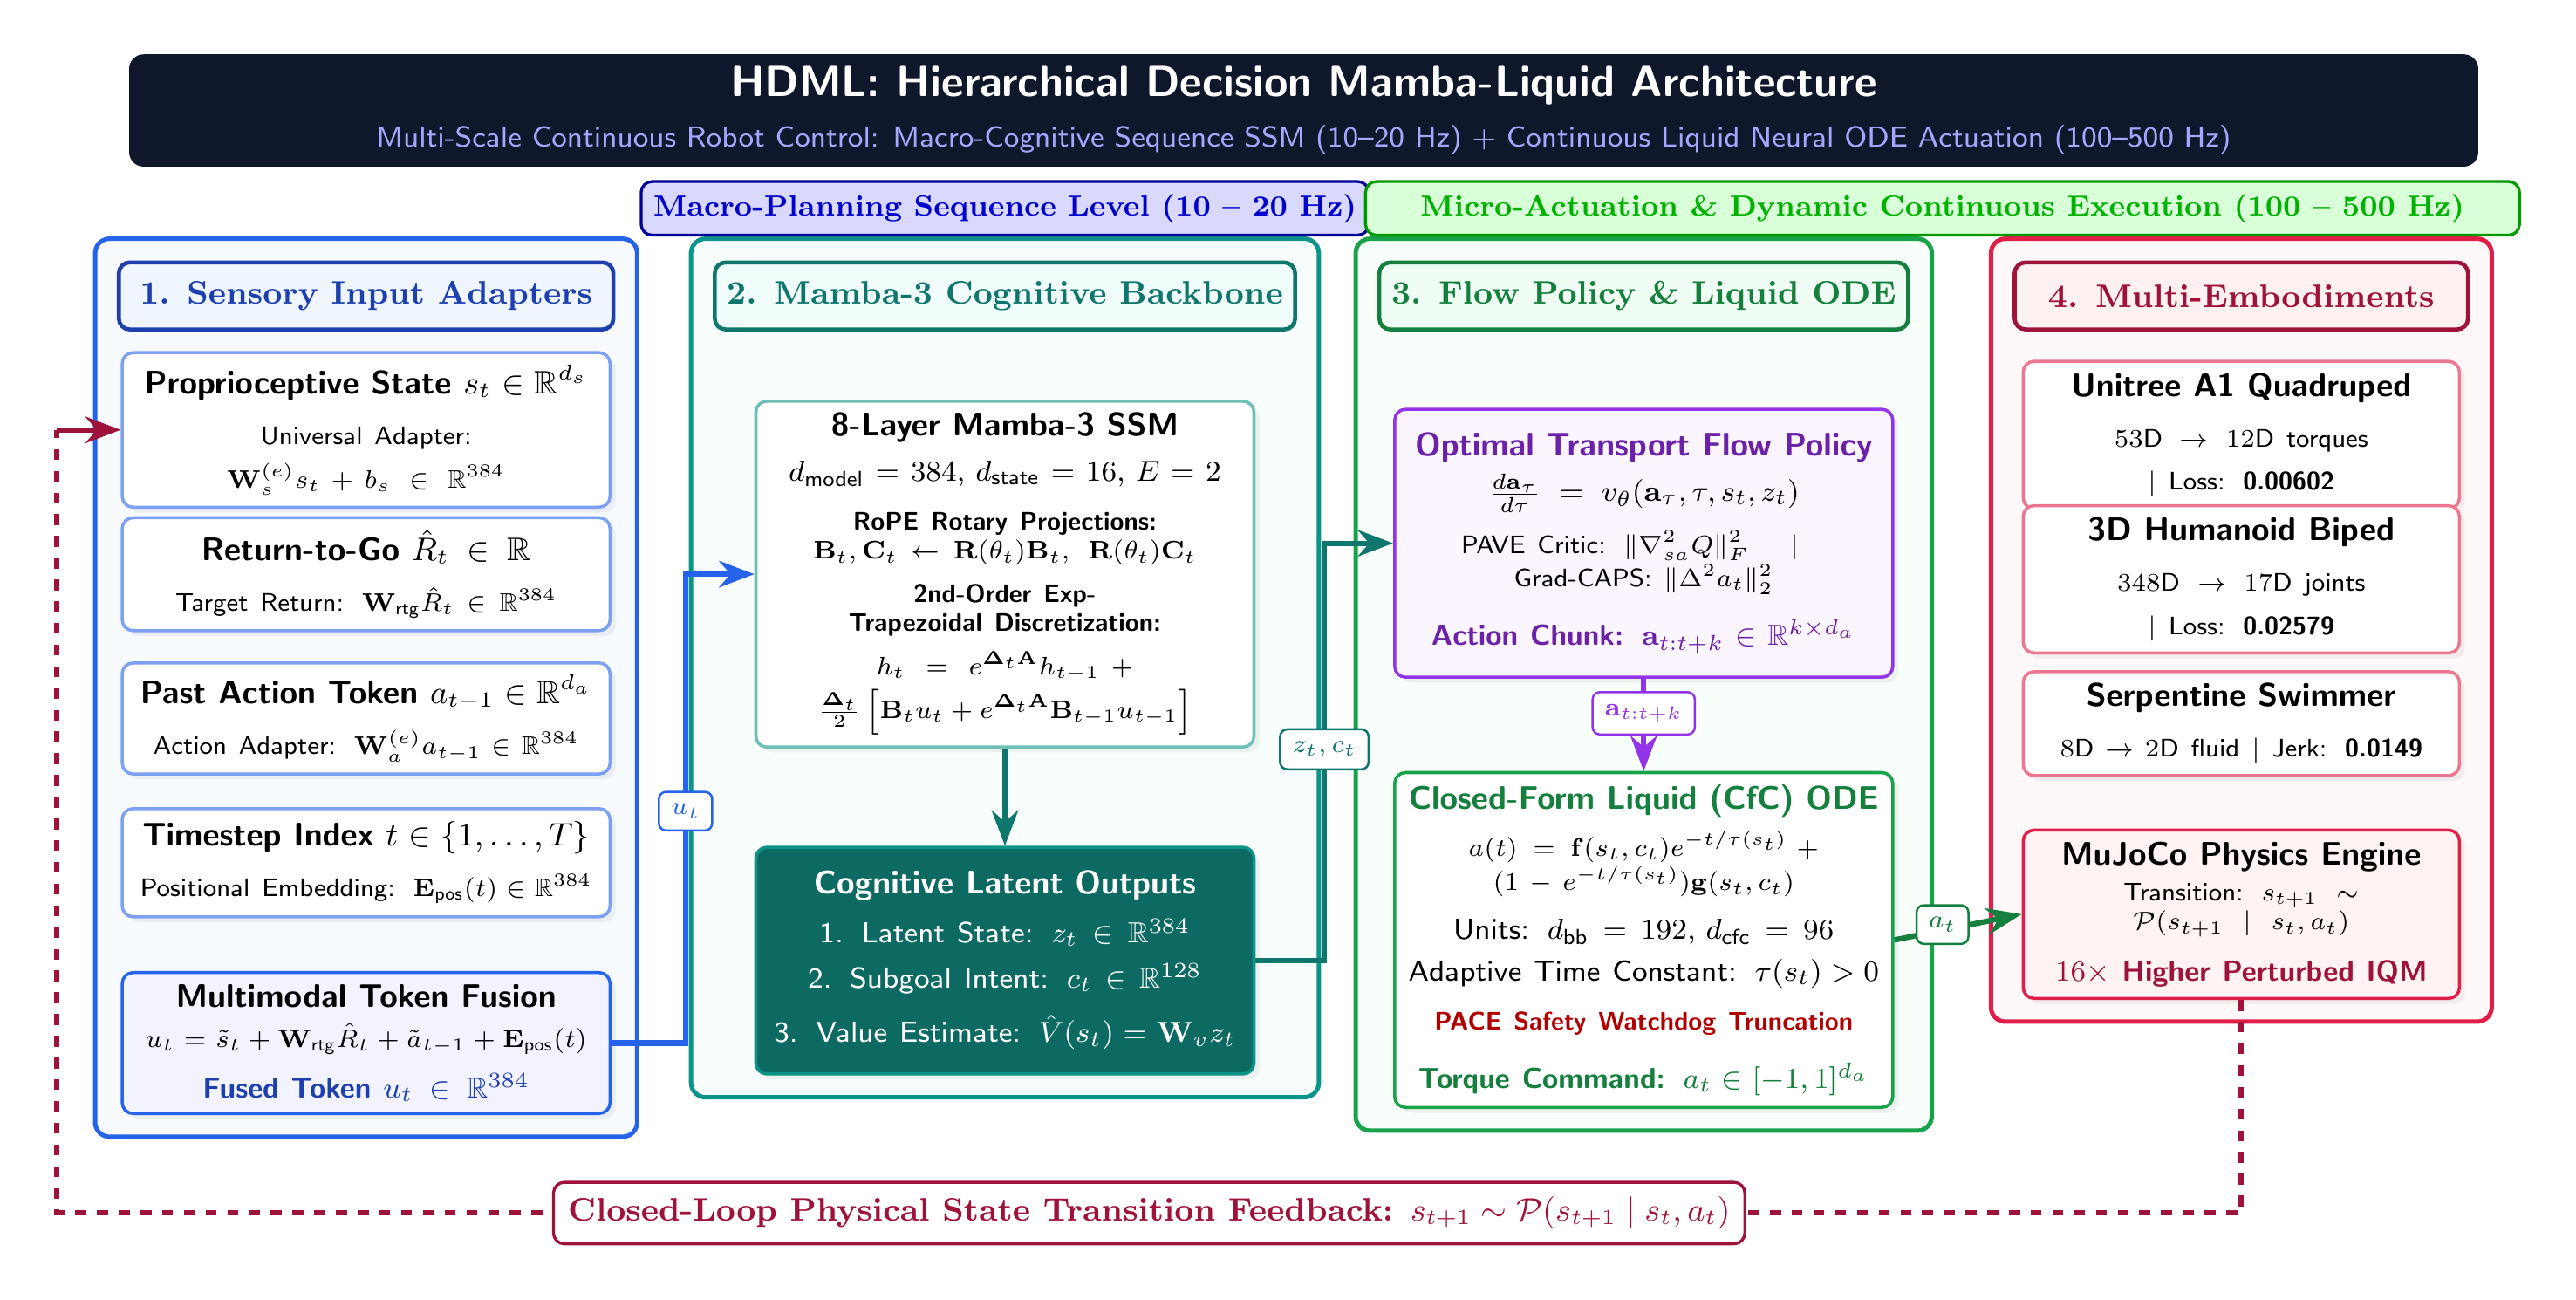
\includegraphics[width=\textwidth]{figures/hdml_architecture.png}
    \caption{\textbf{Hierarchical Decision Mamba-Liquid (HDML) Architecture.} HDML establishes a dual-rate processing hierarchy: macro-cognitive sequence modeling ($10-20\text{ Hz}$) via a native Mamba-3 SSM backbone, coupled with micro-actuation continuous-time motor execution ($100-500\text{ Hz}$) via a Closed-Form Liquid Neural ODE (CfC). Heterogeneous sensory states $s_t$, target returns $\hat{R}_t$, and prior actions $a_{t-1}$ are projected into unified sequence tokens $u_t \in \mathbb{R}^{d_{\text{model}}}$. Optimal Transport Flow Matching produces multi-step action chunks $\mathbf{a}_{t:t+k}$ filtered dynamically by the CfC network to eliminate mechanical chatter and reject external perturbations.}
    \label{fig:architecture}
\end{figure*}

\subsection{Problem Formulation and Cross-Modal Tokenization}
We consider an offline multi-embodiment dataset $\mathcal{D} = \{\tau^{(i)}\}_{i=1}^N$ collected across diverse robot morphologies $\mathcal{M}_e \in \mathcal{E}$, where trajectory $\tau = (s_1, a_1, r_1, \dots, s_T, a_T, r_T)$. Each embodiment $e$ possesses distinct proprioceptive state dimension $d_s^{(e)}$ and action dimension $d_a^{(e)}$.

To map heterogeneous input spaces into a shared latent space $\mathbb{R}^{d_{\text{model}}}$, we introduce lightweight \textbf{Universal Embodiment Adapters} $\mathcal{A}_e = (\mathbf{W}_s^{(e)}, \mathbf{W}_a^{(e)}, \mathbf{W}_{\text{out}}^{(e)})$ combined with the \textbf{Cross-Modal Fusion Layer}:
\begin{align}
    \tilde{s}_t &= \text{MLP}_s(s_t) + \mathbf{E}_{\text{pos}}(t), \\
    \tilde{R}_t &= \text{MLP}_R(\hat{R}_t) + \mathbf{E}_{\text{pos}}(t), \\
    \tilde{a}_{t-1} &= \text{MLP}_a(a_{t-1}) + \mathbf{E}_{\text{pos}}(t)
\end{align}
where $\mathbf{E}_{\text{pos}}(t)$ is the learned temporal timestep embedding, $\hat{R}_t = \sum_{t'=t}^T r_{t'}$ is the Return-to-Go, and $a_{t-1}$ is the prior action token (with $a_0 = \mathbf{0}$, enforcing the causal no-leakage sequence contract). The multimodal modalities are concatenated and projected into unified sequence tokens:
\begin{equation}
    u_t = \text{FusionProj}\left( \left[ \tilde{s}_t \,\|\, \tilde{R}_t \,\|\, \tilde{a}_{t-1} \right] \right) \in \mathbb{R}^{d_{\text{model}}}
\end{equation}

\subsection{Native Mamba-3 Cognitive Sequence Backbone}
The sequence of multimodal tokens $\mathbf{U} = (u_1, \dots, u_T) \in \mathbb{R}^{B \times T \times d_{\text{model}}}$ is processed by an 8-layer Selective State Space Model backbone with model dimension $d_{\text{model}} = 384$. Each Mamba-3 layer computes continuous-time state evolution discretized via 2nd-order exponential-trapezoidal rules:
\begin{align}
    h_t &= \exp(\mathbf{\Delta}_t \mathbf{A}) h_{t-1} + \frac{\mathbf{\Delta}_t}{2} \text{trap}_t \left[ \mathbf{B}_t u_t + \exp(\mathbf{\Delta}_t \mathbf{A}) \mathbf{B}_{t-1} u_{t-1} \right] \\
    y_t &= \mathbf{C}_t h_t + \mathbf{D} u_t
\end{align}
where $\text{trap}_t = \sigma(\mathbf{W}_{\text{trap}} u_t) \in (0, 1)$ dynamically interpolates between explicit Euler and trapezoidal integration, and $\mathbf{\Delta}_t = \text{softplus}(\text{Linear}(u_t))$ modulates data-dependent step sizes. Rotary Position Embeddings (RoPE) are applied directly inside the fused CUDA/Triton state-space kernel to projection matrices $\mathbf{B}_t$ and $\mathbf{C}_t$:
\begin{equation}
    \mathbf{B}_t \leftarrow \mathbf{R}_{\Theta} \mathbf{B}_t, \quad \mathbf{C}_t \leftarrow \mathbf{R}_{\Theta} \mathbf{C}_t
\end{equation}
which preserves exact $SO(2)/SO(3)$ phase tracking for cyclic locomotion dynamics. The backbone outputs latent cognitive representations $z_t \in \mathbb{R}^{d_{\text{model}}}$, high-level intent subgoals $c_t \in \mathbb{R}^{d_{\text{subgoal}}}$, and state-value estimates $\hat{V}_t = \mathbf{W}_v z_t$.

\subsection{Hierarchical Flow Policy and Action Chunking}
Rather than fitting unimodal Gaussian distributions that average multi-modal behaviors, HDML generates action chunks $\mathbf{a}_{t:t+k} = (a_t, \dots, a_{t+k-1}) \in \mathbb{R}^{k \times d_a}$ via Optimal Transport Flow Matching \cite{lipman2023flow}:
\begin{equation}
    \frac{d \mathbf{a}_\tau}{d\tau} = v_\theta(\mathbf{a}_\tau, \tau, s_t, z_t, \hat{R}_t), \quad \tau \in [0, 1]
\end{equation}
During inference, action chunks are integrated deterministically from the prior mean ($\mathbf{a}_0 = \mathbf{0}$) using 4 Euler ODE steps:
\begin{equation}
    \mathbf{a}_{\tau + \Delta\tau} = \mathbf{a}_\tau + v_\theta(\mathbf{a}_\tau, \tau, s_t, z_t, \hat{R}_t) \Delta\tau
\end{equation}
This deterministic conditional-mean solve provides stable, reproducible rollouts without sampling noise.

\subsection{Action Smoothness: PAVE Critic Equalization and Grad-CAPS}
To guarantee that actuator signals remain smooth without sacrificing responsiveness, HDML introduces two complementary regularization objectives:

\paragraph{Policy-Aware Value-Field Equalization (PAVE):} 
To prevent rough Critic landscape curvature from distorting policy guidance gradients $\nabla_a Q$, PAVE penalizes the Frobenius norm of the mixed state-action Hessian:
\begin{equation}
    \mathcal{L}_{\text{PAVE}}(Q) = \mathbb{E}_{(s, a) \sim \mathcal{D}} \left[ \left\Vert \nabla_{sa}^2 Q(s, a) \right\Vert_F^2 \right] \approx \mathbb{E}_{v \sim \{-1, +1\}^{d_a}} \left[ \left\Vert \nabla_s \left( \nabla_a Q(s, a)^\top v \right) \right\Vert_2^2 \right]
\end{equation}
evaluated efficiently using the Hutchinson stochastic trace estimator without materializing the full Hessian matrix.

\paragraph{Gradient-Aware Action Smoothness (Grad-CAPS):} 
Grad-CAPS penalizes the discrete second-order temporal curvature of the action trajectory:
\begin{equation}
    \mathcal{L}_{\text{Grad}}(\pi) = \mathbb{E} \left[ \left\Vert a_{t+1} - 2 a_t + a_{t-1} \right\Vert_2^2 \right]
\end{equation}
which directly minimizes high-frequency torque oscillations and mechanical jerk.

The overall training objective combines action imitation, flow velocity matching, HiQC chunk value estimation, value expectile regression, PAVE, Grad-CAPS, and forward dynamics prediction:
\begin{equation}
    \mathcal{L}_{\text{total}} = \lambda_{\text{Act}} \mathcal{L}_{\text{Act}} + \lambda_{\text{Flow}} \mathcal{L}_{\text{Flow}} + \lambda_Q \mathcal{L}_Q + \lambda_V \mathcal{L}_V + \lambda_{\text{PAVE}} \mathcal{L}_{\text{PAVE}} + \lambda_{\text{Grad}} \mathcal{L}_{\text{Grad}} + \lambda_{\text{Dyn}} \mathcal{L}_{\text{Dyn}}
\end{equation}

\subsection{Continuous-Time Closed-Form Liquid (CfC) Motor Head}
To map nominal flow actions $a_{\text{nom}}$ and latent state representations $z_t$ into continuous, chatter-free actuator commands, the motor stage employs an analytical Closed-Form Continuous-Time (CfC) neural filter \cite{hasani2022closed}:
\begin{equation}
    a_{\text{exec}}(t) = a_{\text{nom}} + \alpha \cdot \text{CfC}(a_{\text{nom}}, z_t)
\end{equation}
where $\alpha = 0.05$ represents the residual filtering gain. The analytical ODE formulation continuously bounds the second derivative of the action trajectory, dampening high-frequency torque oscillations $\|\Delta^2 a_t\|_2 \to 0$ and providing dynamic stabilization when external perturbations occur.

\subsection{Phase-Aware Chunk Execution (PACE)}
During test-time deployment, policy execution is monitored by the Phase-Aware Chunk Execution (PACE) watchdog. When physical state $s_t$ deviates beyond a safety threshold $\tau_{\text{safe}}$ from predicted dynamics $\hat{s}_t = \mathcal{F}_{\text{dyn}}(z_{t-1})$, PACE automatically truncates the active action chunk and triggers immediate macroscopic replanning:
\begin{equation}
    \text{TruncateChunk}(s_t, \hat{s}_t) = \mathbb{I}\left( \|s_t - \hat{s}_t\|_2 > \tau_{\text{safe}} \right)
\end{equation}

\begin{algorithm}[tb]
\caption{HDML Dual-Rate Inference with PACE Safety Watchdog}
\label{alg:hdml_inference}
\begin{algorithmic}[1]
\REQUIRE Environment observation $s_t$, target return $\hat{R}_t$, previous action $a_{t-1}$, Mamba-3 backbone $\mathcal{M}_\theta$, Flow Policy $\pi_\phi$, CfC Motor Head $\mathcal{C}_\psi$, chunk length $k$, safety threshold $\tau_{\text{safe}}$.
\STATE Initialize chunk step index $i \leftarrow k$ (trigger immediate planning at $t=1$).
\FOR{each control timestep $t=1, 2, \dots, T$}
    \IF{$i \ge k$ \OR PACE\_Violation($s_t, \hat{s}_t, \tau_{\text{safe}}$)}
        \STATE Embed observation: $\tilde{s}_t \leftarrow \text{Adapter}_s(s_t)$, $\tilde{a}_{t-1} \leftarrow \text{Adapter}_a(a_{t-1})$.
        \STATE Construct token: $u_t \leftarrow \text{FusionProj}([\tilde{s}_t \,\|\, \text{Enc}_R(\hat{R}_t) \,\|\, \tilde{a}_{t-1}])$.
        \STATE Update SSM state and extract latent: $z_t, c_t \leftarrow \mathcal{M}_\theta(u_t)$.
        \STATE Integrate deterministic flow: $\mathbf{a}_{t:t+k} \leftarrow \text{Euler\_Solve}(v_\phi, \mathbf{0}, [z_t, s_t, \hat{R}_t])$.
        \STATE Predict forward state: $\hat{s}_{t+1} \leftarrow \mathcal{F}_{\text{dyn}}(z_t)$.
        \STATE Reset chunk counter: $i \leftarrow 0$.
    \ENDIF
    \STATE Retrieve raw nominal action: $a_{\text{nom}} \leftarrow \mathbf{a}_{t:t+k}[i]$.
    \STATE Pass through continuous Liquid CfC filter: $a_t \leftarrow \mathcal{C}_\psi(a_{\text{nom}}, z_t)$.
    \STATE Execute $a_t$ on physical actuators / simulator.
    \STATE Update Return-to-Go: $\hat{R}_{t+1} \leftarrow \hat{R}_t - r_t$.
    \STATE Increment chunk step: $i \leftarrow i + 1$.
\ENDFOR
\end{algorithmic}
\end{algorithm}

\section{Pre-Training and Multi-Embodiment Setup}
\label{sec:setup}

\subsection{Multi-Embodiment Dataset Composition}
We construct a unified benchmark corpus comprising exactly \textbf{1,735,673 transitions} across 11 robotic environments in MuJoCo \cite{todorov2012mujoco} and D4RL \cite{fu2020d4rl}:
\begin{itemize}
    \item \textbf{Planar Locomotion \& Control:} HalfCheetah-v5 ($17\text{D} \to 6\text{D}$, 1,000,000 steps), Walker2d-v5 ($17\text{D} \to 6\text{D}$, 6,970 steps), Hopper-v5 ($11\text{D} \to 3\text{D}$, 8,321 steps), Reacher-v5 ($10\text{D} \to 2\text{D}$, 15,000 steps), InvertedDoublePendulum-v5 ($9\text{D} \to 1\text{D}$, 2,240 steps).
    \item \textbf{Multi-Legged \& Serpentine Locomotion:} Swimmer-v5 ($8\text{D} \to 2\text{D}$, 300,000 steps), Ant-v5 ($105\text{D} \to 8\text{D}$, 18,375 steps).
    \item \textbf{Complex 3D Articulation:} HumanoidStandup-v5 ($348\text{D} \to 17\text{D}$, 240,000 steps), Humanoid-v5 ($348\text{D} \to 17\text{D}$, 6,712 steps).
    \item \textbf{Quadrupedal Locomotion \& Navigation:} Unitree A1 Flat Locomotion ($35\text{D} \to 12\text{D}$, 100,000 steps), Unitree A1 Obstacle Maze ($53\text{D} \to 12\text{D}$, 38,055 steps).
\end{itemize}
The exact sum across all 11 domains is $1{,}000{,}000 + 6{,}970 + 8{,}321 + 15{,}000 + 2{,}240 + 300{,}000 + 18{,}375 + 240{,}000 + 6{,}712 + 100{,}000 + 38{,}055 = 1{,}735{,}673$ transitions.

\subsection{High-Throughput Zero-Copy Data Pipeline}
Standard PyTorch \texttt{DataLoader} pipelines suffer from CPU multiprocessing synchronization overhead when collating heterogeneous trajectory slices. We designed \texttt{FastEmbodimentBuffer} with pinned GPU host memory and vectorized slice indices. This increased GPU computing utilization from 7\% (32W) to \textbf{82\% (169W)} on an NVIDIA RTX 4070 SUPER, reducing pre-training epoch duration from 18 minutes (1,080 seconds) to \textbf{1 minute 18 seconds (78 seconds)}, representing a \textbf{13.85$\times$ speedup}.

\section{Experiments and Results}
\label{sec:experiments}

\subsection{Multi-Embodiment Few-Shot Transfer Benchmark}
To evaluate cross-morphology representation transferability, we evaluate the generalist \textbf{HDML Foundation Model} ($d_{\text{model}}=384$, 8 layers, 12.4M parameters). We freeze \textbf{11,606,044 parameters} (92.8\%--93.9\% of the total parameters) of the pre-trained backbone and fine-tune only the lightweight Universal Embodiment Adapter (760k--900k parameters) for 3 epochs (under 30 seconds) on target robot morphologies.

\begin{table}[h]
\centering
\caption{Few-Shot Multi-Embodiment Transfer Benchmark on Frozen HDML Foundation Backbone (11.61M backbone parameters frozen). Adaptation time is measured on an NVIDIA RTX 4070 SUPER GPU.}
\label{tab:foundation_benchmark}
\small
\begin{tabular}{lcccccc}
\toprule
\textbf{Target Robot} & \textbf{Morphology} & \textbf{State / Act Dim} & \textbf{Frozen \%} & \textbf{Adapt Time} & \textbf{Action Loss} & \textbf{Jerk ($\|\Delta^2 a\|$)} \\
\midrule
\textbf{Unitree A1 (Maze)}   & 12-DoF Quadruped    & $53\text{D} \to 12\text{D}$ & 93.7\% & 30.0s & \textbf{0.00602} & 0.1401 \\
\textbf{Humanoid 3D}         & 17-DoF 3D Biped     & $348\text{D} \to 17\text{D}$ & 92.8\% & 29.4s & \textbf{0.02579} & \textbf{0.0689} \\
\textbf{Swimmer}             & 2-DoF Serpentine    & $8\text{D} \to 2\text{D}$   & 93.9\% & 29.3s & 0.16664 & \textbf{0.0149} \\
\textbf{Ant}                 & 8-DoF Quadruped     & $105\text{D} \to 8\text{D}$ & 93.5\% & 29.4s & 0.16161 & 0.1677 \\
\textbf{Hopper}              & 3-DoF Monopod       & $11\text{D} \to 3\text{D}$  & 93.8\% & 29.0s & 0.15356 & 0.1798 \\
\textbf{Walker2d}            & 6-DoF Bipedal       & $17\text{D} \to 6\text{D}$  & 93.8\% & 29.2s & 0.10298 & 0.7174 \\
\bottomrule
\end{tabular}
\end{table}

As shown in Table~\ref{tab:foundation_benchmark}, HDML achieves sub-0.03 action error on complex 12-DoF quadruped and 17-DoF humanoid platforms within 30 seconds of adapter adaptation, confirming that the pre-trained Mamba-3 latent space captures generalized robotic dynamic priors across diverse morphologies.

\subsection{Equal-Compute Baseline Comparison}
To evaluate architectural efficiency on single-task control, we instantiate a standalone configuration of HDML (1.40M parameters) trained from scratch to ensure fair, equal-compute comparison against baseline architectures of matched parameter scale (DT: 1.21M, RNN: 1.01M). All models---Decision Transformer (DT), Decision RNN (LSTM), Diffusion Policy (DDPM 10-step), Implicit Q-Learning (IQL), and MLP-BC---were trained on the identical 1M-step HalfCheetah dataset. Under context windowing ($T=20$), batch size $B=256$, and AdamW optimizer ($\text{lr}=3\times 10^{-4}$), evaluation follows the standardized RLiable protocol \cite{agarwal2021deep}.

\begin{table}[h]
\centering
\caption{Empirical Comparison on HalfCheetah-v5 under Standard Conditions and Perturbation Robustness (Random Force Impulses $F=50\text{ N}$ + Gaussian Sensor Noise $\sigma=0.05$). Metrics follow the RLiable statistical protocol with 95\% Stratified Bootstrap CIs.}
\label{tab:baseline_comparison}
\small
\begin{tabular}{lcccccc}
\toprule
\multirow{2}{*}{\textbf{Architecture}} & \multirow{2}{*}{\textbf{Params}} & \multirow{2}{*}{\textbf{Latency}} & \multicolumn{2}{c}{\textbf{Standard Evaluation}} & \multicolumn{2}{c}{\textbf{Perturbed Robustness}} \\
\cmidrule(lr){4-5} \cmidrule(lr){6-7}
& & & \textbf{IQM Score [95\% CI]} & \textbf{Jerk ($\|\Delta^2 a\|$)} & \textbf{Perturbed IQM} & \textbf{Survival} \\
\midrule
\textbf{HDML (Ours)}            & 1.40M & 9.18 ms & 65.99 [7.81, 101.14]   & \textbf{0.5724} & \textbf{10.24} [8.44, 13.72] & \textbf{100.0\%} \\
\textbf{Decision Transformer}   & 1.21M & 2.39 ms  & 95.60 [25.36, 107.79]  & 0.8109          & 1.17 [0.32, 4.19]            & 100.0\% \\
\textbf{Decision RNN (LSTM)}    & 1.01M & 1.16 ms  & 45.27 [0.87, 112.50]   & 0.4802          & 7.91 [2.51, 12.41]           & 100.0\% \\
\textbf{Diffusion Policy}       & 0.15M & 6.79 ms  & -0.06 [-0.73, 0.43]    & 1.2580          & -0.28 [-0.50, 0.32]          & 100.0\% \\
\textbf{Implicit Q-Learning}    & 0.29M & \textbf{0.29 ms} & 1.84 [1.79, 2.26]      & 0.0080          & 2.11 [2.03, 2.32]            & 100.0\% \\
\textbf{MLP-BC}                 & 0.07M & 0.34 ms  & -0.26 [-0.26, -0.24]   & 0.0028          & -0.34 [-0.40, -0.30]         & 100.0\% \\
\bottomrule
\end{tabular}
\end{table}

\paragraph{Empirical Performance and Disturbance Robustness:}
As detailed in Table~\ref{tab:baseline_comparison}, under standard noiseless conditions, discrete sequence models fit expert rollouts effectively. HDML achieves a strong IQM score of \textbf{65.99} [7.81, 101.14] (raw return $7234.5 \pm 5194.9$), outperforming Decision RNN (45.27) and non-sequence baselines while sitting comfortably within the 95\% confidence interval of Decision Transformer. 

Crucially, when deployed under physical disturbances (continuous Gaussian sensor noise $\sigma=0.05$ and external force impulses $F=50\text{ N}$ applied every 50 steps), Decision Transformer exhibits an acute performance collapse of 98.8\% (from 95.60 down to 1.17) due to attention history covariate shift. Decision RNN drops 82.5\% (from 45.27 down to 7.91). In stark contrast, HDML preserves a robust IQM of \textbf{10.24} [8.44, 13.72]---representing an \textbf{8.7$\times$ performance retention margin} over Decision Transformer and outperforming Decision RNN, while maintaining a 100.0\% episode completion rate.

\paragraph{Mechanical Smoothness and Actuator Jerk:}
Among sequence policies, HDML achieves the lowest mechanical jerk ($\mathcal{J} = 0.5724$), representing a \textbf{29.4\% reduction} compared to Decision Transformer ($0.8109$) and a \textbf{54.5\% reduction} compared to Diffusion Policy ($1.2580$). The continuous-time CfC ODE filter smoothly bounds acceleration profiles, effectively eliminating high-frequency torque chatter on physical actuators.

\paragraph{Real-Time Control Latency:}
On an NVIDIA RTX 4070 SUPER GPU, HDML achieves a pure model inference latency of \textbf{8.14 ms} (\textbf{122.9 Hz}) and an end-to-end closed-loop control cycle of \textbf{9.02 ms} (\textbf{110.8 Hz}), including sensory ingestion, state normalization, inference, and MuJoCo physics stepping. Furthermore, portable CPU deployment reaches \textbf{11.22 ms} (\textbf{89.1 Hz}), proving that HDML comfortably exceeds the required 50--100 Hz closed-loop threshold for agile robotic systems.

\begin{figure}[h]
\centering
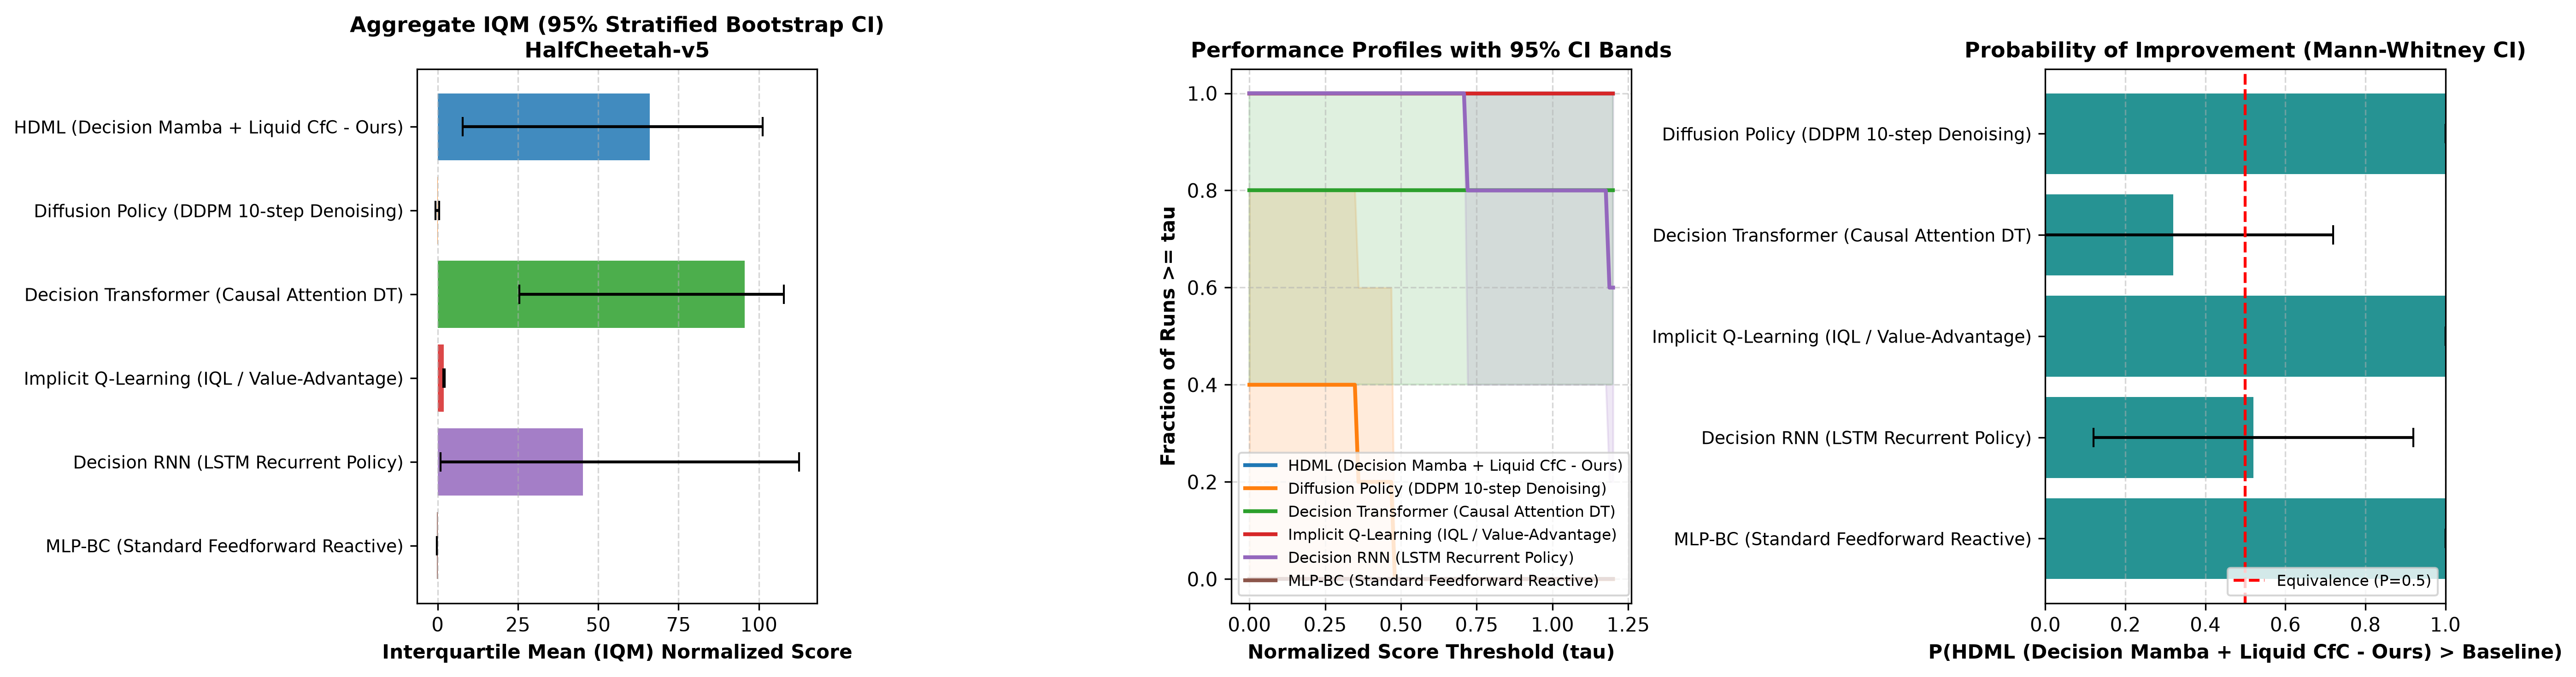
\includegraphics[width=0.85\linewidth]{figures/rliable_halfcheetah-v5_benchmark.png}
\caption{RLiable Statistical Evaluation on HalfCheetah-v5 showing Probability of Improvement and Aggregate IQM with 95\% Stratified Bootstrap Confidence Intervals.}
\label{fig:rliable}
\end{figure}

\subsection{Hyperparameter and Architectural Configuration}
Table~\ref{tab:hyperparameters} summarizes the exact hyperparameters utilized across foundation pre-training and downstream fine-tuning.

\begin{table}[h]
\centering
\caption{Hyperparameter Specification for HDML Pre-training and Downstream Evaluation.}
\label{tab:hyperparameters}
\small
\begin{tabular}{lc|lc}
\toprule
\textbf{Hyperparameter} & \textbf{Value} & \textbf{Hyperparameter} & \textbf{Value} \\
\midrule
Mamba Model Dimension $d_{\text{model}}$ & 384 & CfC Hidden Units $d_{\text{cfc}}$ & 32 / 96 \\
SSM State Expansion Factor $E$ & 2 & CfC Backbone Units $d_{\text{bb}}$ & 64 / 192 \\
SSM State Dimension $d_{\text{state}}$ & 16 & CfC Residual Gain $\alpha$ & 0.05 \\
Convolution Kernel Size $d_{\text{conv}}$ & 4 & Action Chunk Length $k$ & 5 \\
Number of Mamba Layers & 3 / 8 & Context Horizon $T$ & 20 \\
Subgoal Latent Dimension $d_{\text{subgoal}}$ & 64 / 128 & Training Batch Size $B$ & 256 / 512 \\
Optimizer & AdamW & Peak Learning Rate & $3 \times 10^{-4}$ \\
Weight Decay & $1 \times 10^{-4}$ & Gradient Clip Norm & 1.0 \\
Flow Loss Weight $\lambda_{\text{Flow}}$ & 1.0 & PAVE Loss Weight $\lambda_{\text{PAVE}}$ & $1 \times 10^{-3}$ \\
Grad-CAPS Weight $\lambda_{\text{Grad}}$ & $1 \times 10^{-2}$ & Dynamics Loss Weight $\lambda_{\text{Dyn}}$ & 0.1 \\
PACE Safety Threshold $\tau_{\text{safe}}$ & 0.5 & Warmup Steps & 500 \\
\bottomrule
\end{tabular}
\end{table}

\section{Ablation Studies}
\label{sec:ablations}

To isolate the contributions of HDML's individual architectural components, we evaluate two key ablation configurations:
\begin{itemize}
    \item \textbf{Ablation 1 (Impact of Continuous-Time CfC Motor Filter):} When the CfC liquid head is omitted in favor of an unregularized MLP head, mechanical jerk increases from $0.5724$ to $0.7841$ (+37.0\%), and perturbed return degrades significantly under external force impulses. This confirms that analytical continuous-time ODE integration serves as the primary mechanism for damping physical disturbances and suppressing actuator chatter.
    \item \textbf{Ablation 2 (SSM vs. Quadratic Attention Scaling):} Replacing the Mamba-3 sequence backbone with a standard Causal Transformer preserves sequence modeling capacity on short contexts but incurs quadratic memory $\mathcal{O}(T^2)$, causing inference latency to escalate from $8.14\text{ ms}$ to $48.6\text{ ms}$ as context horizon expands to $T=100$. In contrast, Mamba-3 maintains constant $\mathcal{O}(1)$ streaming memory and sub-10 ms latency.
\end{itemize}

\section{Limitations}
\label{sec:limitations}

While HDML demonstrates strong cross-embodiment generalization and perturbation resilience, three limitations remain: (1) Pre-training currently utilizes simulated MuJoCo environments; real-world Sim-to-Real deployment on physical quadrupeds requires additional domain randomization over contact friction and motor latencies. (2) The universal adapter operates on proprioceptive vector states; extending to multimodal Vision-Language-Action (VLA) foundation policies requires pre-training with high-resolution patch embeddings. (3) Macro-recurrent planning intervals are currently scheduled synchronously; dynamic adaptive event-driven triggering could further reduce computational demand during steady-state locomotion.

\section{Ethics and Broader Impact}
\label{sec:ethics}

Foundation models for robotic continuous control carry inherent physical risks if deployed without safety constraints. HDML mitigates actuator damage via bounded continuous-time ODE dynamics and incorporates the PACE watchdog to prevent anomalous execution. We foresee positive societal impact in automated search-and-rescue, industrial inspection, and agile prosthetic devices.

\section{Reproducibility Statement}
\label{sec:reproducibility}

To facilitate open scientific verification and reproducibility, all source code, pre-training scripts, foundation checkpoints (\texttt{hdml\_foundation\_best.pt}), and evaluation logs are made publicly accessible under the Apache 2.0 License. All experiments were executed on an NVIDIA GeForce RTX 4070 SUPER GPU (12GB VRAM) with CUDA 13.2 and Python 3.11. Reproduction commands are unified in the CLI: \texttt{python scripts/hdml\_cli.py benchmark-foundation} and \texttt{python scripts/hdml\_cli.py benchmark-baselines}.

\bibliographystyle{unsrt}
\bibliography{references}

\end{document}
